\section{Σήματα εισόδου} \label{sec:input_signals}

\noindent
Τα πηγαία σήματα που χρησιμοποιήθηκαν για την εκπαίδευση των NN ήταν 'εκρήξεις' (bursts) λευκού θορύβου, ο οποίος έχει χαρακτηριστικά που περιγράφονται στην υποενότητα \ref{sec:white_noise}. Συνολικά η διάρκεια κάθε σήματος ήταν $200 ms$. Στην περίπτωση της δειγματοληψίας με $f_s = 44.1 kHz$ αυτό αντιστοιχεί σε 8820 δείγματα. Οι εκρήξεις είχαν μεταβλητή διάρκεια $3 - 170 ms$ με τυχαίο τρόπο. Τυχαίο ήταν επίσης το σημείο εκκίνησης της κάθε έκρηξης στο συνολικό σήμα. Δημιουργήθηκαν συνολικά 29 τέτοια σήματα και η γενική περιγραφή κάθε σήματος φαίνεται στην εξίσωση \ref{eq:input_signals}, όπου $Z_n \sim N(0,P)$ δηλαδή μια κανονική κατανομή με μέση τιμή μηδέν και διακύμανση-ισχύ \textit{P}.

\begin{CEquation}
\begin{split}
         Sig_in(n) = 
         \begin{cases}
         Z_n, & n_{start} < n < n_{end}\\
         0, & \text{αλλού}
         \end{cases}   
         \label{eq:input_signals}
\end{split}
\end{CEquation}

Μερικά από τα σήματα εισόδου φαίνονται στο Σχήμα \ref{fig:input_signals_examples}. Μετά την δημιουργία τους κανονικοποιούνται στο κλειστό διάστημα $amplitude = [-1, 1]$, ώστε τελικά να αποθηκευτούν σε μορφή wav για μελλοντική χρήση. Η διάρκεια των σημάτων καθορίστηκε στα $200 ms$, προκειμένου να διατηρηθεί σχετικά μικρό το διάνυσμα εισόδου στο NN, αλλά και να προλάβει να επέλθει η σταθερή κατάσταση μετά τη μεταβατική κατάσταση (transient) που δημιουργείται στην έναρξη και την παύση του σήματος, αφού κρίθηκε πως αυτό έχει ιδιαίτερη σημασία στον τρόπο που αντιλαμβάνεται ο άνθρωπος τον ήχο, και άρα να τροφοδοτηθεί το NN, με δεδομένα που έχουν υψηλή συγκέντρωση χρήσιμης πληροφορίας.

\begin{figure}[h]
  \centering
  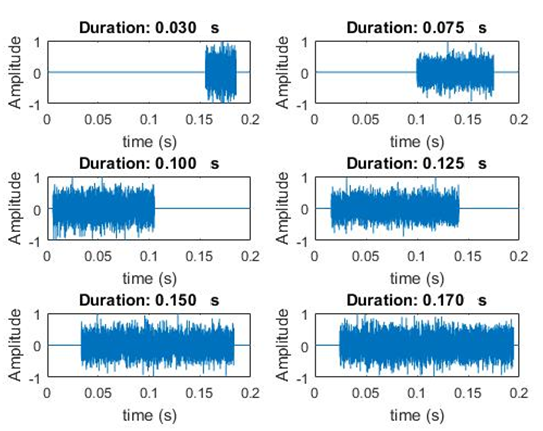
\includegraphics[width=\textwidth]{images/bursts.png}
  \caption{Σήματα λευκού θορύβου που χρησιμοποιήθηκαν ως είσοδος στο μοντέλο.}
  \label{fig:input_signals_examples}
\end{figure}

